% ===== handout mode =====
% Comment/uncomment this line to toggle handout mode
% \newcommand{\handout}{}

% Comment/uncoment this line to toogle Mortitz mode
% \newcommand{\Moritz}{}

% Comment/uncomment this line to toggle handout mode
% \newcommand{\handout}{}

% by Stephan

%% Moritz mode or Stephan mode
\ifdefined \MoritzMode

% This is a configuration file with private, tutor specific information.
% It is therefore excluded from the Git repository so changes in this file will not conflict in git commits.

% Copy this Template, rename to config.tex and add your information below.

\newcommand{\mymail}{moritz.laupichler@student.kit.edu} % Consider using your named student Mail address to keep your u-Account private.

\newcommand{\myname}{\href{mailto:\mymail}{Moritz Laupichler}}

\newcommand{\mytutnumber}{27}

\newcommand{\mytutinfos}{Dienstags, 5. Block (15:45-17:15), SR 236}

\newcommand{\aboutMeFrame}{
	\begin{frame}{Euer Tutor}
		Name: \myname \\
		Alter: 19 Jahre \\
		Studiengang: Bachelor Informatik, 3. Semester \\
		\vspace{1cm}
		\pause 
		\centering{Kontakt: \href{mailto:\mymail}{\mymail}}
	\end{frame}
}

% Toggle Handout mode by including the following line before including style_tut
% and removing the % at the start (but do NOT remove it here, otherwise handout mode will always be on!)
% Please keep handout mode on in all commits!

% \newcommand{\handout}{} % Moritz mode
\fi
\ifdefined \AlexMode

% This is a configuration file with private, tutor specific information.
% It is therefore excluded from the Git repository so changes in this file will not conflict in git commits.

% Copy this Template, rename to config.tex and add your information below.

\newcommand{\mymail}{alexander.klug@student.kit.edu} % Consider using your named student Mail address to keep your u-Account private.

\newcommand{\myname}{\href{mailto:\mymail}{Alexander Klug}}

\newcommand{\mytutnumber}{30}

\newcommand{\mytutinfos}{Mittwochs, 3. Block (11:30-13:00), SR -107}

\newcommand{\aboutMeFrame}{
	\begin{frame}{Euer Tutor}
		Name: \myname \\
		Alter: 19 Jahre \\
		Studiengang: Bachelor Informatik, 3. Semester \\
		\vspace{1cm}
		\pause 
		\centering{Kontakt: \href{mailto:\mymail}{\mymail}}
	\end{frame}
}

% Toggle Handout mode by including the following line before including style_tut
% and removing the % at the start (but do NOT remove it here, otherwise handout mode will always be on!)
% Please keep handout mode on in all commits!

% \newcommand{\handout}{} % Alex Mode
\fi
\ifdefined \StephanMode

% This is a configuration file with private, tutor specific information.
% It is therefore excluded from the Git repository so changes in this file will not conflict in git commits.

% Copy this Template, rename to config.tex and add your information below.

\newcommand{\mymail}{stephan.bohr@student.kit.edu} % Consider using your named student Mail address to keep your u-Account private.

\newcommand{\myname}{\href{mailto:\mymail}{Stephan Bohr}}

\newcommand{\mytutnumber}{19}

\newcommand{\mytutinfos}{Dienstags, 3. Block (11:30-13:00), SR -108}

\newcommand{\aboutMeFrame}{
	\begin{frame}{Euer Tutor}
		Name: \myname \\
		Alter: 21 Jahre \\
		Studiengang: Bachelor Informatik, 5. Semester \\
		\vspace{1cm}
		\pause 
		\centering{Kontakt: \href{mailto:\mymail}{\mymail}}
	\end{frame}
} % Stephan mode
\fi

%% Beamer-Klasse im korrekten Modus
\ifdefined \handout
\documentclass[handout]{beamer} % Handout mode
\else
\documentclass{beamer}
\fi
%\documentclass[18pt,parskip]{beamer}

%% SLIDE FORMAT

% use 'beamerthemekit' for standard 4:3 ratio
% for widescreen slides (16:9), use 'beamerthemekitwide'

\usepackage{../templates/KIT-slides/beamerthemekit}
%\usepackage{../templates/KIT-slides/beamerthemekitwide}

%% TITLE PICTURE

% if a custom picture is to be used on the title page, copy it into the 'logos'
% directory, in the line below, replace 'mypicture' with the 
% filename (without extension) and uncomment the following line
% (picture proportions: 63 : 20 for standard, 169 : 40 for wide
% *.eps format if you use latex+dvips+ps2pdf, 
% *.jpg/*.png/*.pdf if you use pdflatex)

\titleimage{../figures/titleimage/brain}

%% TITLE LOGO

% for a custom logo on the front page, copy your file into the 'logos'
% directory, insert the filename in the line below and uncomment it

%\titlelogo{mylogo}

% (*.eps format if you use latex+dvips+ps2pdf,
% *.jpg/*.png/*.pdf if you use pdflatex)

%% TikZ INTEGRATION

% use these packages for PCM symbols and UML classes
% \usepackage{templates/tikzkit}
% \usepackage{templates/tikzuml}

%\usepackage{tikz}
%\usetikzlibrary{matrix}
%\usetikzlibrary{arrows.meta}
%\usetikzlibrary{automata}
%\usetikzlibrary{tikzmark}

%%%%%%%%%%%%%%%%%%%%%%%%%
% Libertine font (Original GBI font)
\usepackage[mono=false]{libertine}
%\renewcommand*\familydefault{\sfdefault}  %% Only if the base font of the document is to be sans serif

%% Schönere Schriften
\usepackage[TS1,T1]{fontenc}

%% Deutsche Silbentrennung und Beschriftungen
\usepackage[ngerman]{babel}

%% UTF-8-Encoding
\usepackage[utf8]{inputenc}

%% Bibliotheken für viele mathematische Symbole
\usepackage{amsmath, amsfonts, amssymb}

%% Anzeigetiefe für Inhaltsverzeichnis: 1 Stufe
\setcounter{tocdepth}{1}

%% Hyperlinks
\usepackage{hyperref}
% I don't know why, but this works and only includes sections and NOT subsections in the pdf-bookmarks.
\hypersetup{bookmarksdepth=subsection}

%% remove navigation symbols
\setbeamertemplate{navigation symbols}{}

%% switch between "ngerman" and "english" for German/English style date and logos
\selectlanguage{ngerman}

%% for invisible pause texts instead of dimming
\setbeamercovered{invisible}

\usepackage[german=swiss]{csquotes}

\usepackage{tabularx}
\usepackage{booktabs}

\usepackage{tikz}


% Problem: disabled itemize-icons
%\usepackage{enumitem}
% %\setlist[enumerate]{topsep=0pt,itemsep=-1ex,partopsep=1ex,parsep=1ex}
% \setlist[itemize]{noitemsep, nolistsep}
% \setlist[enumerate]{noitemsep, nolistsep}

% Mathmode no vertical space (https://tex.stackexchange.com/a/47403/146825)
\setlength{\abovedisplayskip}{0pt}
\setlength{\belowdisplayskip}{0pt}
\setlength{\abovedisplayshortskip}{0pt}
\setlength{\belowdisplayshortskip}{0pt}

%%%%%%%%%%%% Slides %%%%%%%%%%%%%%%%

\newcommand{\Moritz}[1]{
	\ifdefined \MoritzMode
	#1
	\fi
}

\newcommand{\Alex}[1]{
	\ifdefined \AlexMode
	#1
	\fi
}

\newcommand{\Stephan}[1]{
	\ifdefined \StephanMode
	#1
	\fi
}

\newcommand{\notMoritz}[1]{
	\Alex{#1} \Stephan{#1}
}

\newcommand{\notAlex}[1]{
	\Moritz{#1} \Stephan{#1}
}

\newcommand{\notStephan}[1]{
	\Alex{#1} \Moritz{#1}
}

%% Wochennummer
%\newcounter{weeknum}

%% Titelinformationen
%\title[GBI Tutorium, Woche \theweeknum]{Grundbegriffe der Informatik \\ Tutorium \mytutnumber}
%\subtitle{Termin \theweeknum \ | \mydate \\ \myname}
\author[\myname]{\myname}
\institute{Fakultät für Informatik}
%\date{\mydate}

%% Titel einfügen
\newcommand{\titleframe}{\frame{\titlepage}\addtocounter{framenumber}{-1}}


%% Alles starten mit \starttut{X}
%\newcommand{\starttut}[1]{\setcounter{weeknum}{#1}\titleframe\frame{\frametitle{Inhalt}\tableofcontents} \AtBeginSection[]{%
%\begin{frame}
%	\tableofcontents[currentsection]
%\end{frame}\addtocounter{framenumber}{-1}}}


%\newcommand{\framePrevEpisode}{
%	\begin{frame}
%		\centering
%		\textbf{In the previous episode of GBI...}
%	\end{frame}
%}

%% Roadmap frame
%table of contents
\newcommand{\roadmap}{
	\frame{\frametitle{Roadmap}\tableofcontents}}

 \AtBeginSection[]{%
\begin{frame}
	\frametitle{Roadmap}
	\tableofcontents[currentsection]
\end{frame}%\addtocounter{framenumber}{-1}
}


%% ShowMessage frame
\newcommand{\showmessage}[1]{\frame{\frametitle{\phantom{1em}}\centering\textbf{#1}}}

%% Fragen
%% Lastframe
\newcommand{\questionframe}{\showmessage{Fragen?}}

%% Lastframe
\newcommand{\lastframe}{\showmessage{Vielen Dank für Eure Aufmerksamkeit! \\Bis nächste Woche :)}}

%% Thanks frame
\newcommand{\slideThanks}{
	\begin{frame}
		\frametitle{Credits}
		\begin{block}{}
			An der Erstellung des Foliensatzes haben mitgewirkt:\\[1em]
			\Moritz{
			Stephan Bohr \\
			Alexander Klug \\
			}
			\Alex{
			Stephan Bohr \\
			Moritz Laupichler \\
			}
			\Stephan{
			Moritz Laupichler \\
			Alexander Klug \\
			}
			Katharina Wurz \\
			Thassilo Helmold \\
			Daniel Jungkind \\
			% Philipp Basler \\
			% Nils Braun \\
			% Dominik Doerner \\
			% Ou Yue \\
		\end{block}
	\end{frame}
}

%% Verbatim
%\usepackage{moreverb}

% GBI related stuff, but not beamer-stuff
\newcommand{\newpar}[1]{\paragraph{#1}\mbox{}\newline}

\newcommand{\nM}{\mathbb{M}}
\newcommand{\nR}{\mathbb{R}}
\newcommand{\nN}{\mathbb{N}}
\newcommand{\nZ}{\mathbb{Z}}
\newcommand{\nQ}{\mathbb{Q}}
\newcommand{\nB}{\mathbb{B}}
\newcommand{\nC}{\mathbb{C}}
\newcommand{\nK}{\mathbb{K}}
\newcommand{\nF}{\mathbb{F}}
\newcommand{\nG}{\mathbb{G}}
\newcommand{\nullel}{\mathcal{O}}
\newcommand{\einsel}{\mathds{1}}
\newcommand{\nP}{\mathbb{P}}
\newcommand{\Pot}{\mathcal{P}}
\renewcommand{\O}{\text{O}}

\newcommand{\bfmod}{\ensuremath{\text{\textbf{ mod }}}}
\renewcommand{\mod}{\bfmod}
\newcommand{\bfdiv}{\ensuremath{\text{\textbf{ div }}}}
\renewcommand{\div}{\bfdiv}


\newcommand{\set}[1]{\left\{ #1 \right\}}
\newcommand{\setc}[2]{\set{#1 \mid #2}}
\newcommand{\setC}[2]{\set{#1 \mid \text{ #2 }}}

\newcommand{\setsize}[1]{\; \mid #1 \mid \; }

\newcommand{\q}[1]{\textquotedblleft #1\textquotedblright}

% Zu zeigen, thx to http://www.matheboard.de/archive/155832/thread.html
\newcommand{\zz}{\ensuremath{\mathrm{z\kern-.29em\raise-0.44ex\hbox{z}}}:}

% Text above symbol
% https://tex.stackexchange.com/a/74132/146825
%
% \newcommand{\eqtext}[1]{\stackrel{\mathclap{\normalfont\mbox{#1}}}{=}}
% \newcommand{\gdwtext}[1]{\stackrel{\mathclap{\normalfont\mbox{#1}}}{\Leftrightarrow}}
% \newcommand{\imptext}[1]{\stackrel{\mathclap{\normalfont\mbox{#1}}}{\Rightarrow}}
% \newcommand{\symbtext}[2]{\stackrel{\mathclap{\normalfont\mbox{#2}}}{#1}}
\newcommand{\eqtext}[1]{\mathrel{\overset{\makebox%[0pt]
{\mbox{\normalfont\tiny #1}}}{=}}}
\newcommand{\gdwtext}[1]{\mathrel{\overset{\makebox%[0pt]
{\mbox{\normalfont\tiny #1}}}{\ensuremath{\Leftrightarrow}}}}
\newcommand{\imptext}[1]{\mathrel{\overset{\makebox%[0pt]
{\mbox{\normalfont\tiny #1}}}{\ensuremath{\Rightarrow}}}}
\newcommand{\symbtext}[2]{\mathrel{\overset{\makebox%[0pt]
{\mbox{\normalfont\tiny #2}}}{#1}}}

% qed symbol
\newcommand{\qedblack}{\hfill \ensuremath{\blacksquare}}
\newcommand{\qedwhite}{\hfill \ensuremath{\Box}}

% Aussagenlogik
% Worsch
\colorlet{alcolor}{blue}
\RequirePackage{tikz}
\usetikzlibrary{arrows.meta}
\newcommand{\alimpl}{\mathrel{\tikz[x={(0.1ex,0ex)},y={(0ex,0.1ex)},>={Classical TikZ Rightarrow[]}]{\draw[alcolor,->,line width=0.7pt,line cap=round] (0,0) -- (15,0);\path (0,-6);}}}
\newcommand{\alimp}{\alimpl}
\newcommand{\aleqv}{\mathrel{\tikz[x={(0.1ex,0ex)},y={(0ex,0.1ex)},>={Classical TikZ Rightarrow[]}]{\draw[alcolor,<->,line width=0.7pt,line cap=round] (0,0) -- (18,0);\path (0,-6);}}}
\newcommand{\aland}{\mathbin{\raisebox{-0.6pt}{\rotatebox{90}{\texttt{\color{alcolor}\char62}}}}}
\newcommand{\alor}{\mathbin{\raisebox{-0.8pt}{\rotatebox{90}{\texttt{\color{alcolor}\char60}}}}}
%\newcommand{\ali}[1]{_{\mathtt{\color{alcolor}#1}}}
\newcommand{\alv}[1]{\mathtt{\color{alcolor}#1}}
\newcommand{\alnot}{\mathop{\tikz[x={(0.1ex,0ex)},y={(0ex,0.1ex)}]{\draw[alcolor,line width=0.7pt,line cap=round,line join=round] (0,0) -- (10,0) -- (10,-4);\path (0,-8) ;}}}
\newcommand{\alP}{\alv{P}} %ali{#1}}
%\newcommand{\alka}{\negthinspace\hbox{\texttt{\color{alcolor}(}}}
\newcommand{\alka}{\negthinspace\text{\texttt{\color{alcolor}(}}}
%\newcommand{\alkz}{\texttt{\color{alcolor})}}\negthinspace}
\newcommand{\alkz}{\text{\texttt{\color{alcolor})}}\negthinspace}

% Thassilo
\newcommand{\BB}{\mathbb{B}}
\newcommand{\boder}{\alor}%{\ensuremath{\text{\;}\textcolor{blue}{\vee}}\text{\;}}
\newcommand{\bund}{\aland}%{\ensuremath{\text{\;}\textcolor{blue}{\wedge}}\text{\;}}
\newcommand{\bimp}{\alimp}%{\ensuremath{\text{\;}\textcolor{blue}{\to}}\text{\;}}
\newcommand{\bnot}{\alnot}%{\ensuremath{\text{\;}\textcolor{blue}{\neg}}\text{}}
\newcommand{\bgdw}{\aleqv}%{\ensuremath{\text{\;}\textcolor{blue}{\leftrightarrow}}\text{\;}}
\newcommand{\bone}{\ensuremath{\textcolor{blue}{1}}\text{}}
\newcommand{\bzero}{\ensuremath{\textcolor{blue}{0}}\text{}}
\newcommand{\bleftBr}{\alka}%{\ensuremath{\textcolor{blue}{(}}\text{}}
\newcommand{\brightBr}{\alkz}%{\ensuremath{\textcolor{blue}{)}}\text{}}

\newcommand{\val}{\hbox{\textit{val}}}

\newcommand{\VarAL}{\hbox{\textit{Var}}_{AL}}
\newcommand{\ForAL}{\hbox{\textit{For}}_{AL}}

% Validierungsfunktion val_i
\newcommand{\vali}[1]{\ensuremath{\val_I(#1)}}

% Boolsche Funktion b_
\newcommand{\bfnot}[1]{\ensuremath{b_{\bnot}(#1)}}
\newcommand{\bfand}[2]{\ensuremath{b_{\bund}(#1,#2)}}
\newcommand{\bfor}[2]{\ensuremath{b_{\boder}(#1,#2)}}
\newcommand{\bfimp}[2]{\ensuremath{b_{\bimp}(#1,#2)}}

% Aussagenkalkül
\newcommand{\AAL}{A_{AL}}
\newcommand{\LAL}{\hbox{\textit{For}}_{AL}}
\newcommand{\AxAL}{\hbox{\textit{Ax}}_{AL}}
\newcommand{\MP}{\hbox{\textit{MP}}}

% Prädikatenlogik
% die nachfolgenden Sachen angepasst an cmtt
\newlength{\ttquantwd}
\setlength{\ttquantwd}{1ex}
\newlength{\ttquantht}
\setlength{\ttquantht}{6.75pt}
\def\plall{%
  \tikz[line width=0.67pt,line cap=round,line join=round,baseline=(B),alcolor] {
    \draw (-0.5\ttquantwd,\ttquantht) -- node[coordinate,pos=0.4] (lll){} (-0.25pt,-0.0pt) -- (0.25pt,-0.0pt) -- node[coordinate,pos=0.6] (rrr){} (0.5\ttquantwd,\ttquantht);
    \draw (lll) -- (rrr);
    \coordinate (B) at (0,-0.35pt);
  }%
}
\def\plexist{%
  \tikz[line width=0.67pt,line cap=round,line join=round,baseline=(B),alcolor] {
    \draw (-0.9\ttquantwd,\ttquantht) -- (0,\ttquantht) -- node[coordinate,pos=0.5] (mmm){} (0,0) --  (-0.9\ttquantwd,0);
    \draw (mmm) -- ++(-0.75\ttquantwd,0);
    \coordinate (B) at (0,-0.35pt);
  }\ensuremath{\,}%
}
\let\plexists=\plexist
\newcommand{\NT}[1]{\ensuremath{\langle\mathrm{#1} \rangle}}
\newcommand{\CPL}{\text{\itshape Const}_{PL}}
\newcommand{\FPL}{\text{\itshape Fun}_{PL}}
\newcommand{\RPL}{\text{\itshape Rel}_{PL}}
\newcommand{\VPL}{\text{\itshape Var}_{PL}}
\newcommand{\plka}{\alka}
\newcommand{\plkz}{\alkz}
%\newcommand{\plka}{\plfoo{(}}
%\newcommand{\plkz}{\plfoo{)}}
\newcommand{\plcomma}{\hbox{\texttt{\color{alcolor},}}}
\newcommand{\pleq}{{\color{alcolor}\,\dot=\,}}

\newcommand{\plfoo}[1]{\mathtt{\color{alcolor}#1}}
\newcommand{\plc}{\plfoo{c}}
\newcommand{\pld}{\plfoo{d}}
\newcommand{\plf}{\plfoo{f}}
\newcommand{\plg}{\plfoo{g}}
\newcommand{\plh}{\plfoo{h}}
\newcommand{\plx}{\plfoo{x}}
\newcommand{\ply}{\plfoo{y}}
\newcommand{\plz}{\plfoo{z}}
\newcommand{\plR}{\plfoo{R}}
\newcommand{\plS}{\plfoo{S}}
\newcommand{\ar}{\mathrm{ar}}

\newcommand{\bv}{\mathrm{bv}}
\newcommand{\fv}{\mathrm{fv}}

\def\word#1{\hbox{\textcolor{blue}{\texttt{#1}}}}
%\let\literal\word
\def\mword#1{\hbox{\textcolor{blue}{$\mathtt{#1}$}}}  % math word
\def\sp{\scalebox{1}[.5]{\textvisiblespace}}
\def\wordsp{\word{\sp}}


\newcommand{\W}{\ensuremath{\hbox{\textbf{w}}}\xspace}
\newcommand{\F}{\ensuremath{\hbox{\textbf{f}}}\xspace}
\newcommand{\WF}{\ensuremath{\{\W,\F\}}\xspace}
\newcommand{\valDIb}{\val_{D,I,\beta}}

\newcommand{\impl}{\ifmmode\ensuremath{\mskip\thinmuskip\Rightarrow\mskip\thinmuskip}\else$\Rightarrow$\fi\xspace}
\newcommand{\Impl}{\ifmmode\implies\else$\Longrightarrow$\fi\xspace}

\newcommand{\derives}{\Rightarrow}

\newcommand{\gdw}{\ifmmode\mskip\thickmuskip\Leftrightarrow\mskip\thickmuskip\else$\Leftrightarrow$\fi\xspace}
\newcommand{\Gdw}{\ifmmode\iff\else$\Longleftrightarrow$\fi\xspace}

\newcommand*{\from}{\colon}
\newcommand{\functionto}{\longrightarrow}


\newcommand{\LTer}{L_{\text{\itshape Ter}}}
\newcommand{\LRel}{L_{\text{\itshape Rel}}}
\newcommand{\LFor}{L_{\text{\itshape For}}}
\newcommand{\NTer}{N_{\text{\itshape Ter}}}
\newcommand{\NRel}{N_{\text{\itshape Rel}}}
\newcommand{\NFor}{N_{\text{\itshape For}}}
\newcommand{\PTer}{P_{\text{\itshape Ter}}}
\newcommand{\PRel}{P_{\text{\itshape Rel}}}
\newcommand{\PFor}{P_{\text{\itshape For}}}

\newcommand{\sgn}{\mathop{\text{sgn}}}

\newcommand{\lang}[1]{\ensuremath{\langle#1\rangle}}

\newcommand{\literal}[1]{\hbox{\textcolor{blue!95!white}{\textup{\texttt{\scalebox{1.11}{#1}}}}}}
\let\hashtag\#
\renewcommand{\#}[1]{\literal{#1}}

\def\blank{\ensuremath{\openbox}}
\def\9{\blank}
\newcommand{\io}{\!\mid\!}


\providecommand{\fspace}{\mathord{\text{space}}}
\providecommand{\fSpace}{\mathord{\text{Space}}}
\providecommand{\ftime}{\mathord{\text{time}}}
\providecommand{\fTime}{\mathord{\text{Time}}}

\newcommand{\fnum}{\text{num}}
\newcommand{\fNum}{{\text{Num}}}

\def\Pclass{\text{\bfseries P}}
\def\PSPACE{\text{\bfseries PSPACE}}



\title[Algorithmen in Graphen, Quantitative Aspekte von Algorithmen]{12. Tutorium\\ Algorithmen in Graphen, \\Quantitative Aspekte von Algorithmen}
\subtitle{Grundbegriffe der Informatik, Tutorium \#\mytutnumber}
\date{\today}


\begin{document}
\titleframe
\roadmap

%%%%%%%%%% %%%%%%%%%%
\section{Algorithmen in Graphen}
\subsection{Wiederholung Adjazenz-/Wegematrix}
\begin{frame}{Wdh.: Adjazenzmatrix}
	\begin{block}{Def.: Adjazenzmatrix}
		\begin{columns}
			\begin{column}{0.475\textwidth}
				Sei $G=(V_G,E_G)$ gerichteter Graph.\\
				\textbf{Adjazenzmatrix} $A \in \set{0,1}^{\mid V_G \mid \times \mid V_G \mid}$\\[12pt]
				\[
					A_{ij} = 
					\begin{cases}
						1, & \text{ falls } (i,j)\in E_G\\
						0, & \text{ falls } (i,j)\notin E_G
					\end{cases}
				\]
			\end{column}
			\begin{column}{0.475\textwidth}
				Sei $U=(V_U,E_U)$ ungerichteter Graph.\\
				\textbf{Adjazenzmatrix} $A \in \set{0,1}^{\mid V_U \mid \times \mid V_U \mid}$\\[12pt]
				\[
					A_{ij} = 
					\begin{cases}
						1, & \text{ falls } \set{i,j}\in E_U\\
						0, & \text{ falls } \set{i,j}\notin E_U
					\end{cases}
				\]
			\end{column}
		\end{columns}
	\end{block}
\pause
	\begin{exampleblock}{Besondere Eigenschaften der Adjazenzmatrix}
		\begin{itemize}
			\item Schlingen lassen sich an einer $1$ auf der Diagonalen erkennen (Wert von $A_{ii}$) 
			\item Bei ungerichteten Graphen ist $A$ immer symmetrisch (also $A_{ij} = A_{ji}$).
		\end{itemize}
	\end{exampleblock}
\end{frame}

\begin{frame}{Wdh.: Wegematrix}
    \begin{block}{Def.: Wegematrix}
		\begin{columns}
			\begin{column}{0.95\textwidth}
				Sei $G=(V_G,E_G)$ gerichteter Graph.\\
				\textbf{Wegematrix} $W \in \set{0,1}^{\mid V_G \mid \times \mid V_G \mid}$\\[12pt]
				\[
					W_{ij} = 
					\begin{cases}
						1, & \parbox[t]{.6\textwidth}{ falls es in $E_G$ Pfad von $i$ nach $j$ gibt.}\\
						0, & \parbox[t]{.6\textwidth}{ sonst}
					\end{cases}
				\]
			\end{column}
		\end{columns}
	\end{block}
\end{frame}
\subsection{Von der Adjazenz- zur Wegematrix, Ausblick Warshall-Algorithmus}
\subsection{Von der Adjazenz- zur Wegematrix, Ausblick Warshall-Algorithmus}
\begin{frame}{Kantenrelation}
	\begin{block}{Kantenmenge als Relation}
		Sei $G$ ein gerichteter Graph mit der Knotenmenge $V$. Die Kantenmenge ist wie folgt definiert:\\
		Sei $E \subseteq V \times V$ eine Relation auf $V$ definiert durch $(x,y) \in E \gdw \text{es gibt eine Kante von $x$ nach }y \text{ in } G$.
	\end{block}

	\begin{exampleblock}{Beobachtungen}
		\begin{itemize}
			\item Was gilt für $E^2$? \pause $\Rightarrow$ Knoten, die über einen Pfad der Länge 2 verbunden sind
			\item Analog $E^3$, $E^4$, \dots
			\item Also $(x,y) \in E^*$ genau dann, wenn es einen Pfad (beliebiger Länge) von $x$ nach $y$ gibt.
		\end{itemize}
	\end{exampleblock}
\end{frame}

\begin{frame}{Berechnung der Erreichbarkeitsrelation}
    \begin{block}{Erreichbarkeitsrelation}
        Sei $n = |V|$
    	\[
    		E^* = \bigcup_{i=0}^{\infty} E^i = \bigcup_{i=0}^{n-1} E^i
    	\]
    \end{block}

    \begin{block}{Matrizen für die Relation $E^k$}
    	Sei $G$ ein gerichteter Graph mit Adjazenzmatrix $A$. Für alle $k \in \nN_0$ gilt:\\
    	\[
    		\sgn((A^k)_{ij}):=
    		\begin{cases}
      		1 & \text{ falls in $G$ ein Pfad der Länge $k$ von $i$ nach $j$ existiert}\\
      		0 & \text{ falls in $G$ kein Pfad der Länge $k$ von $i$ nach $j$ existiert}\\
    		\end{cases}
    	\]
    \end{block}
\end{frame}

\begin{frame}{Berechnung der Wegematrix}	
    \begin{block}{Berechnung der Wegematrix}
    	Es sei $G$ ein gerichteter Graph mit Adjazenzmatrix $A$. Dann gilt für alle $k\geq n-1$: 
    	\[
    		W = \sgn\left(\sum_{i=0}^{k} A^i\right) 
    	\]
    	ist die Wegematrix des Graphen $G$.
    \end{block}
\end{frame}


\section{Quantitative Aspekte von Algorithmen}
\newcommand{\Rplus}{\ensuremath{\nR_+}}
\newcommand{\Rnullplus}{\ensuremath{\nR^+_0}}
\subsection{Ressourcenverbrauch, Abängigkeit von n, Best- Worst- und Average-Case}
\begin{frame}{Laufzeit}
\centering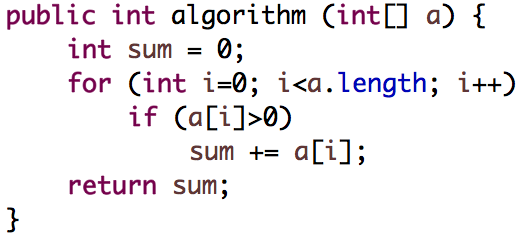
\includegraphics[height=4cm]{algorithm}

\begin{exampleblock}{Aufgabe}
	Wie viele \emph{Instruktionen} werden aufgerufen? \\% Worst-Case: n+1, Best-Case: 1, Average Case ?
	\pause
	Im \emph{worst case}? Im \emph{best case}? Im \emph{average case}?
\end{exampleblock}
\end{frame}
\subsection{O-Kalkül}
\begin{frame}{O-Notation}
	\begin{block}{Def. Asymptotisches Wachstum $\asymp$}
		Seien $f,g \from \nN_0 \to \Rnullplus$. Dann gilt
		\[
			f \asymp g \Leftrightarrow \exists c,c'\in \Rplus: \exists n_0\in \nN_0: \forall n\geq n_0: c f(n) \leq g(n) \leq c' f(n)
		\]
		Man sagt auch $g$ wächst genauso schnell wie $f$. $\asymp$ ist eine Äquivalenzrelation.
	\end{block}

	\begin{exampleblock}{Beispiele}
		\begin{itemize}
			\item $42n^6-33n^3+222n^2 -15 \asymp 66n^6+55555n^5$
			\item $n^{3+1}+5n^2\asymp 3n^3-n$
		\end{itemize}
	\end{exampleblock}
\end{frame}

\begin{frame}{$O$-Notation}
    \begin{block}{$\Theta$-Kalkül}
    	\begin{align*}
  			\Theta(f) &= \{ g \mid f \asymp g \} \\
  				   &= \{ g \mid \exists c,c'\in \Rplus: \exists n_0\in \nN_0: \forall  n\geq n_0: c f(n) \leq g(n) \leq c' f(n) \} 
		\end{align*}
    \end{block}

    \begin{exampleblock}{Bemerkungen}
    	\begin{itemize}
    		\item Im $\Theta$-Kalkül von $f(n)$ sind genau die Funktionen enthalten, die asymptotisch gleich schnell wachsen wie $f(n)$.
    		\item Schreibe $g(n) \in \Theta(f(n))$, wenn $g(n)$ asymptotisch gleichschnell wächst wie $f(n)$.
    		\item Ist $f$ ein Polynom, so sind insbesondere in $\Theta(f(n))$ alle Polynome enthalten, die den gleichen Grad wie $f$ haben.
    		\item Es gilt $\log_b(n) \in\Theta(\log_a(n))$. Die Basis ist also egal und man kann auch $\Theta(\log n)$ schreiben. % TODO Aufgabe und Beweis hierzu
    		% TODO Theta ist != Average Case
    	\end{itemize}
    \end{exampleblock}
\end{frame}

\begin{frame}{$O$-Notation}
    \begin{block}{Def.: $O$-Kalkül}
    	\[
    		O(f) = \{ g \mid \exists c\in \Rplus:\exists n_0\in\nN_0: \forall n\geq n_0: g(n) \leq c f(n)\}
    	\]

    	$g(n) \in O(f(n))$ (oder $g \preceq f$) genau dann, wenn $g$ asymptotisch höchstens so schnell wächst wie $f$.
    \end{block}
\pause
    \begin{block}{Def.: $\Omega$-Kalkül}
    	\[
    		\Omega(f) = \{ g \mid \exists c\in \Rplus:\exists n_0\in\nN_0: \forall n\geq n_0: g(n) \geq c f(n)\}
    	\]
    	
    	$g(n) \in \Omega(f(n))$ (oder $g \succeq f$) genau dann, wenn $g$ asymptotisch mindestens so schnell wächst wie $f$.
    \end{block}
\pause
    Beobachtung: $\Theta(f) = O(f) \cap \Omega(f)$
\end{frame}

\begin{frame}{$O$-Notation}
	\begin{exampleblock}{Aufgabe}
		\begin{enumerate}
			\item Für welches $c \in \Rplus$ gilt $5n^4 \in O(n^c)$ bzw $5n^4 \in \Omega(n^c)$?
			\item Für welches $c \in \Rplus$ gilt $5n^4 \in O(c^n)$ bzw $5n^4 \in \Omega(c^n)$?
			\item Für welches $c \in \Rplus$ gilt $2^n \in O(c^n)$ bzw $2^n \in \Omega(c^n)$?
			\item Zeige oder widerlege: $n \in \Theta(\sqrt{n})$
		\end{enumerate}
	\end{exampleblock}
\pause
	\begin{block}{Lösung}
		\begin{enumerate}
			\item Es gilt: $\forall c \geq 4$ bzw. $\forall c \leq 4$.
			\item Es gilt: $\forall c > 1$ bzw. $\forall c \leq 1$.
			\item Es gilt: $\forall c \geq 2$ bzw. $\forall c \leq 2$.
			\item \small Annahme: Die Behauptung ist richtig.\\
				Dann gilt: $n \in O(\sqrt{n}) \wedge n \in \Omega(\sqrt{n})$, insbesondere $n \in \Omega(\sqrt{n})$.\\
				$\Rightarrow \exists c\in \Rplus:\exists n_0\in\nN_0: \forall n\geq n_0: n \leq c \sqrt{n} \Leftrightarrow \frac{n}{\sqrt{n}} \leq c \Leftrightarrow \sqrt{n} \leq c$. Widerspruch.
				
		\end{enumerate}
	\end{block}
\end{frame}

\begin{frame}{$O$-Notation}
    \begin{exampleblock}{Aufgabe}
    	Zeige oder widerlege:
    	\[
    		f(n) + g(n) \in O(g(f(n)))
    	\]
    \end{exampleblock}
\pause
	\begin{block}{Lösung}
		Die Behauptung stimmt nicht. Wähle z.B. $f(n) = n^2$ und $g(n) = \sqrt{n}$ und führe dies zu einem Widerspruch.
	\end{block}
\end{frame}

\begin{frame}{$O$-Notation} % TODO: Logarithmusregeln, Typische Abschätzungskette (1 < log n < sqrt(n) < n < n log n < n c (c>1) < c^n < n!)
    \begin{itemize}
    	\item $\Theta$ entspricht \emph{nicht} dem average case.
    	\item $O(1)$ bedeutet konstante Laufzeit
    	\item Beachtet den \emph{Trick} mit den Limites\footnote{Ich weiß nicht, ob ihr den als Beweis in der Klausur oder auf dem Blättern verwenden dürft. Zur Kontrolle sollte man ihn aber kennen.}
        \item Es gilt mit Konstante $c \in \Rplus$ mit $c>1$
        \[
            1 \preceq \log n \preceq \sqrt{n} \preceq n \preceq n \log n \preceq n^c \preceq c^n \preceq n!
        \]
        \nachgucken https://martin-thoma.com/die-landau-symbole/
    \end{itemize}
\end{frame}


\subsection{Master-Theorem}
\begin{frame}{Mastertheorem}
    \textbf{Problemstellung:}\\[1cm]    
    Gegeben sei eine \emph{rekursiv} definierte Funktion $T$.\\
    Frage: Welche Laufzeit hat $T$?\\[1cm]
    Beispiel:
    \[
    	T(n) = 8 T \left(\frac{n}{2} \right) + 1000n^2
    \]
    \\[1cm]\centering$\Rightarrow$ \emph{Mastertheorem}
\end{frame}

\begin{frame}{Mastertheorem}
    \begin{block}{Def.: Mastertheorem}
    	Seien $a\geq 1$ und $b>1$ Konstanten, $f \from \nN \to \Rnullplus$ und $T(n)$ eine Laufzeitfunktion der Form
    	\[
			T = a T\left(\frac{n}{b}\right) + f 
		\]
		Dann gilt nach dem \textbf{Mastertheorem}:
		\begin{itemize}
			\item \textbf{Fall 1:} \\ Wenn $f \in O(n^{\log_b a -\varepsilon})$ für ein $\varepsilon>0$ ist, dann ist $T\in \Theta(n^{\log_b a})$.
			\item \textbf{Fall 2:} \\ Wenn $f \in \Theta(n^{\log_b a})$ ist, dann ist $T\in \Theta(n^{\log_b a}\log n)$.
			\item\textbf{Fall 3:} \\  Wenn $f \in \Omega(n^{\log_b a +\varepsilon})$ für ein $\varepsilon>0$ ist, und wenn es eine Konstante $d$ gibt mit $0<d<1$, so dass für alle hinreichend großen $n$ gilt $af\left(\frac{n}{n}\right)\leq d f$, dann ist $T\in \Theta(f)$.
		\end{itemize}
    \end{block}
\end{frame}

\begin{frame}{Mastertheorem}
    \begin{exampleblock}{Beispiel zum 1. Fall}
    	Sei $T(n) = 8 T \left(\frac{n}{2} \right) + 1000n^2$.
    	\begin{itemize}
    		\item Aus der Formel lässt sich ablesen:\\
    			$a=8$, $b=2$, $f(n)=1000n^2$
    		\item $n^{\log_b a}$ bestimmen:\\
    			$\log_b a = \log_2 8 = 3 \Rightarrow n^{\log_b a} = n^3$
    		\item $n^{\log_b a}$ mit $f(n)$ vergleichen: $1000n^2 \in O(n^3-\varepsilon)$?\\
    			Ja, für $\varepsilon = 1$ gilt $1000n^2 \in O(n^2)$.
    		\item Mit dem Mastertheorem folgt:\\
    			$T(n) = \Theta(n^3)$
    	\end{itemize}
    \end{exampleblock}
\end{frame}


\begin{frame}{Mastertheorem}
    \begin{exampleblock}{Beispiel zum 2. Fall}
    	Sei $T(n) = 2 T \left(\frac{n}{2} \right) + 10n$.
    	\begin{itemize}
    		\item Aus der Formel lässt sich ablesen:\\
    			$a=2$, $b=2$, $f(n)=10n$
    		\item $n^{\log_b a}$ bestimmen:\\
    			$\log_b a = \log_2 2 = 1 \Rightarrow n^{\log_b a} = n^1$
    		\item $n^{\log_b a}$ mit $f(n)$ vergleichen: $10n \in \Theta(n)$?\\
    			Ja!
    		\item Mit dem Mastertheorem folgt:\\
    			$T(n) = \Theta(n \log n)$
    	\end{itemize}
    \end{exampleblock}
\end{frame}



\begin{frame}{Mastertheorem}
    \begin{exampleblock}{Beispiel zum 3. Fall}
    	Sei $T(n) = 2 T \left(\frac{n}{2} \right) + n^2$.
    	\begin{itemize}
    		\item Aus der Formel lässt sich ablesen:\\
    			$a=2$, $b=2$, $f(n)=n^2$
    		\item $n^{\log_b a}$ bestimmen:\\
    			$\log_b a = \log_2 2 = 1 \Rightarrow n^{\log_b a} = n^1$
    		\item $n^{\log_b a}$ mit $f(n)$ vergleichen: $n^2 \in \Omega(n^{1+\varepsilon})$?\\
    			Ja, für $\varepsilon = 1$ gilt $n^2 \in \Omega(n^2)$.
    		\item Zusatzbedingung überprüfen: Ist $af\left(\frac{n}{n}\right)\leq d f$?\\
    			Ja, für $d = \frac{1}{2}$ gilt $\forall n \geq 1 \; : \; \frac{1}{2}n^2 \leq \frac{1}{2}n^2$
    		\item Mit dem Mastertheorem folgt:\\
    			$T(n) = \Theta(n^2)$
    	\end{itemize}
    \end{exampleblock}
\end{frame}


%%%%%%%%%% %%%%%%%%%%
%% Zusammenfassung
\section{}
%\subsection{Zusammenfassung}
	\begin{frame}{Was ihr jetzt kennen und können solltet\dots}
			\begin{itemize}
				\item Von der \emph{Adjazenzmatrix} zur \emph{Wegematrix}
				\item \emph{Laufzeiten} von Algorithmen angeben und abschätzen
				\item Mit dem \emph{$O$-Kalkül} arbeiten
				\item Die Laufzeit rekursiver Algorithmen mit dem \emph{Mastertheorem} bestimmen
			\end{itemize}
	
	\end{frame}
%% Ausblick
%\subsection{Ausblick}
	\begin{frame}{Ausblick}
		\begin{itemize}
			\item Erste Nutzung von Graphen: \emph{endliche Automaten}
			\item Neue Möglichkeiten mit formalen Sprachen: \emph{reguläre Ausdrücke} und \emph{rechtslineare Grammatriken} 
		\end{itemize}
	\end{frame}
%%%%%%%%%% %%%%%%%%%%
\section{}
\questionframe
\lastframe
\mode<handout>{\slideThanks}
\end{document}